\documentclass[12pt]{article}
\usepackage[pdfborder={0 0 0.5 [3 2]}]{hyperref}%
\usepackage[left=1in,right=1in,top=1in,bottom=1in]{geometry}%
\usepackage[shortalphabetic]{amsrefs}%
\usepackage{amsmath}
\usepackage{enumerate}
\usepackage{enumitem}
\usepackage{amssymb}                
\usepackage{amsmath}                
\usepackage{amsfonts}
\usepackage{amsthm}
\usepackage{bbm}
\usepackage[table,xcdraw]{xcolor}
\usepackage{tikz}
\usepackage{float}
\usepackage{booktabs}
\usepackage{svg}
\usepackage{mathtools}
\usepackage{cool}
\usepackage{url}
\usepackage{graphicx,epsfig}
\usepackage{framed}
\usepackage{hyperref}  

\usetikzlibrary{automata,arrows,positioning,calc}
\DeclarePairedDelimiter\abs{\lvert}{\rvert}%
\DeclarePairedDelimiter\norm{\lVert}{\rVert}%
\DeclarePairedDelimiter\ceil{\lceil}{\rceil}
\DeclarePairedDelimiter\floor{\lfloor}{\rfloor}

\makeatletter
\renewcommand*\env@matrix[1][*\c@MaxMatrixCols c]{%
  \hskip -\arraycolsep
  \let\@ifnextchar\new@ifnextchar
  \array{#1}}
\makeatother

\newtheorem{theorem}{Theorem}[section]
\newtheorem{corollary}{Corollary}[theorem]
\newtheorem{proposition}[theorem]{Proposition}
\newtheorem{lemma}[theorem]{Lemma}

\theoremstyle{definition}
\newtheorem{definition}[theorem]{Definition}
\newtheorem{exercise}{Exercise}%
\newtheorem{problem}[exercise]{Problem}%
\newtheorem*{example}{Example}

\theoremstyle{remark}
\newtheorem*{question}{Question}
\newtheorem*{observation}{Observation}
\newtheorem*{remark}{Remark}

\graphicspath{ {images/} }

\setlength{\parindent}{0cm}
\renewcommand{\vec}[1]{\ensuremath{\mathbf{#1}}}

\def\noi{\noindent}
\def\T{{\mathbb T}}
\def\R{{\mathbb R}}
\def\N{{\mathbb N}}
\def\C{{\mathbb C}}
\def\Z{{\mathbb Z}}
\def\P{{\mathbb P}}
\def\E{{\mathbb E}}
\def\Q{\mathbb{Q}}
\def\ind{{\mathbb I}}

\def\cale{{\mathcal E}}
\def\cals{{\mathcal S}}
\def\calc{{\mathcal C}}
\def\caln{{\mathcal N}}
\def\calb{{\mathcal B}}
\def\calg{{\cal G}}

\def\ds{\displaystyle}
\def\ra{\rightarrow}
\newcommand{\conv}{\mbox{\rm conv}}
\newcommand{\spaan}{\mbox{\rm span}}
\newcommand{\deet}{\mbox{\rm det}}
\newcommand{\aff}{\mbox{\rm aff}}
\newcommand{\cl}{\mbox{\rm cl}}
\newcommand{\dimm}{\mbox{\rm dim}}
\newcommand{\sm}{\setminus}
\def\ci{\perp\!\!\!\perp}

\newcommand{\ink}{\rule{.5\baselineskip}{.55\baselineskip}}

\begin{document}

\setcounter{section}{5}
\section{Estimation}

\subsection{Introduction}
The purpose of statistics is to make inferences about populations based on data from a small sample of that population. Populations are characterized by probability distributions which can be described by numerical parameters. The population mean $\mu$ and population variance $\sigma^2$ are parameters common to all probability distributions. In addition, some populations can be described by other natural parameters. One example is the population of all registered voters in Rhode Island. If we are interested in the yes/no question ``Are you going to vote for Gina Raimondo?'', a natural parameter is $p$, the proportion of the population who plans on voting for Raimondo.\\

The setup is exactly the same as with sampling. Suppose we are studying a population whose distribution is characterized by a parameter of interest which we will denote $\theta$ (this could be the population mean, population variance, proportion of voters supporting Raimondo, or some other parameter). We will take $n$ independent, identically distributed samples $Y_1, \dots, Y_n$ from our population. An \emph{estimator} is a function of our $n$ samples which is designed to give us information about the population parameter. There are two types of estimators we will discuss:
\begin{enumerate}
\item A \emph{point estimator} produces a single number which we think is close to the parameter of interest. We will learn several ways to quantitatively evaluate the ``goodness'' of a point estimator
\item An \emph{interval estimate} produces an interval (often called a confidence interval) in which we believe our parameter of interest lies. We will learn how to construct confidence intervals which include the parameter of interest with a given probability.
\end{enumerate}


\subsection{Point Estimators}
We start our discussion with point estimators. We have already met one point estimator, the sample mean $\bar{Y}$. The sample mean is an estimator since it is a function of our $n$ samples. It is an estimator for the population mean. For another example, suppose we are polling $n$ voters out of a population of registered voters and asking them if they are voting for Gina Raimondo. The parameter of interest is $p$, the proportion of registered voters who will vote for Raimondo. Let $Y$ be the number of voters in our sample who are voting for Raimondo. Then the sample proportion $\hat{p} = Y/n$ is an estimator for the population proportion $p$. (The ``hat'' over the $p$ indicates that it is an estimator for the parameter $p$).\\

Since we are applied mathematicians, we need quantitative tools to tell whether an estimator is any good. Let $\hat{\theta}$ be an estimator for the parameter $\theta$. The first criterion we can use to evaluate an estimator is \emph{bias}. We would like the expected value of our estimator to be the actual value of the parameter we are trying to estimate, i.e. $\E(\hat{\theta}) = \theta$. An estimator which has this property is called \emph{unbiased}

\begin{framed}
\emph{Bias of an Estimator}\\
  \rule{\dimexpr\linewidth-2\fboxsep-2\fboxrule}{.1pt} \\
Let $\hat{\theta}$ be an estimator for a parameter $\theta$. The estimator $\hat{\theta}$ is \emph{unbiased} if $\E(\hat{\theta}) = \theta$. Otherwise, the estimator $\hat{\theta}$ is \emph{biased}. The \emph{bias} of $\hat{\theta}$ is given by
\[
Bias(\hat{\theta}) = \E(\hat{\theta}) - \theta
\]
\end{framed}

Let's look at the estimators we have seen so far. The sample mean $\bar{Y}$ is an estimator for the population mean $\mu$ (here we abandon our ``hat''-convention, and call this $\bar{Y}$ rather than $\hat{\mu}$). We showed in the last section that $\E(\bar{Y}) = \mu$, thus the sample mean is an unbiased estimator for the population mean.\\

What about the sample proportion estimator we use in polling? Suppose we poll $n$ voters in a population, and let $Y$ be the number of voters in our sample who are voting for Gina Raimondo. As long as the sample is small enough (less than 1/20 of the population size), we can take $Y$ to be a binomial random variable with parameters $n$ and $p$. For our estimator $\hat{p} = Y/n$, 
\[
\E(\hat{p}) = \E\left( \frac{Y}{n} \right) = \frac{1}{n}\E(Y) = \frac{np}{n} = p
\]
where we have used the expected value of a binomial random variable. Since $\E(\hat{p}) = p$, this estimator is unbiased as well. We will see an example of a biased estimator later.\\

A perhaps better measure of the ``goodness'' of an estimator is its \emph{mean square error}, the average of the square distance of the estimator from the parameter of interest.

\begin{framed}
\emph{Mean Square Error}\\
  \rule{\dimexpr\linewidth-2\fboxsep-2\fboxrule}{.1pt} \\
Let $\hat{\theta}$ be an estimator for a parameter $\theta$. The \emph{mean square error} of $\hat{\theta}$ is defined by
\[
MSE(\hat{\theta}) = \E[ (\hat{\theta} - \theta)^2]
\]
If $Bias(\hat{\theta})$ is the bias of $\hat{\theta}$ and $Var(\hat{\theta})$ is the variance of $\hat{\theta}$, then
\[
MSE(\hat{\theta}) = [Bias(\hat{\theta})]^2 + Var(\hat{\theta})
\] 
\end{framed}
Note that the MSE can be divided into two components: variance and bias squared. Both of these are positive. We have discussed above how low bias is a good quality for an estimator. Low variance is a desired quality for an estimator as well since ideally we would like the distribution of the estimator to cluster tightly about the parameter of interest. In general, if we keep the sample size fixed, there is a tradeoff between bias and variance. For a given MSE, if we wish our estimator to have lower bias, then we must accept a higher variance and vice versa.\\

To show the relationship between MSE, bias, and variance, we take the definition of MSE and add and subtract $\E(\hat{\theta})$ inside the parentheses.

\begin{align*}
MSE(\hat{\theta}) &= \E[ (\hat{\theta} - \theta)^2 ] \\
&= \E[ (\hat{\theta} - \E(\hat{\theta})) + (\E(\hat{\theta}) - \theta)]^2 \\
&= \E[ (\hat{\theta} - \E(\hat{\theta}))^2] + 2 \E [ (\hat{\theta} - \E(\hat{\theta})) (\underbrace{\E(\hat{\theta}) - \theta)}_{\text{constant}} ] + \E[ \underbrace{(\E(\hat{\theta}) - \theta)^2}_{\text{constant}} ] \\
&= Var(\hat{\theta} ) + 2 (\E(\hat{\theta}) - \theta) \E [ (\hat{\theta} - \E(\hat{\theta})) ] + (\E(\hat{\theta}) - \theta)^2\\
&= Var(\hat{\theta} ) + 2 (\E(\hat{\theta}) - \theta) (\underbrace{\E(\hat{\theta}) - \E(\hat{\theta})}_{=0}) + [Bias(\hat{\theta})]^2 \\
&= Var(\hat{\theta} ) + [Bias(\hat{\theta})]^2
\end{align*}

Let's look at the MSE of the two estimators we discussed above.
\begin{enumerate}
\item Sample mean $\bar{Y} = \frac{1}{n}\sum_{i=1}^n Y_i$\\

We showed that this estimator is unbiased, so the MSE is equal to the variance. We showed in a previous section that the variance of the sample mean is $\sigma^2 / n$, where $\sigma^2$ is the population variance. Thus we have
\[
MSE(\bar{Y}) = \frac{\sigma^2}{n}
\]
Note that the MSE goes to 0 as $n \rightarrow \infty$, i.e. the error of our estimator decreases as our sample gets larger. This makes intuitive sense that a larger sample provides a better estimator for the population mean.

\item Sample proportion. $\hat{p} = \frac{Y}{n}$. \\

Recall that we are assuming that $Y \sim\text{ Binomial}(n, p)$. We showed above that this estimator is also unbiased, thus once again the MSE is equal to the variance. Recalling that the variance of a binomial random variable is $np(1-p)$,
\begin{align*}
MSE(\hat{p}) &= Var\left(\frac{Y}{n}\right) \\
&= \frac{1}{n^2} Var(Y) \\
&= \frac{np(1-p)}{n^2}\\
&= \frac{p(1-p)}{n}
\end{align*}

\end{enumerate}

Sometimes we are interested in studying the difference between two populations. Here are some examples of that.

\begin{enumerate}
\item Suppose we are interested in whether Brown University first-year students or seniors get more sleep. In this case, the parameter of interest is the \emph{difference} in the mean amount of sleep between first-years and seniors. If $\mu_1$ and $\sigma^2_1$ are the mean and variance of the amount of sleep of first-years and $\mu_2$ and $\sigma^2_2$ are the same for seniors, then mathematically our parameter of interest is $\mu_1 - \mu_2$. If we take a sample of $n_1$ first-year students and $n_2$ seniors and compute the sample means $\bar{Y}_1$ and $\bar{Y}_2$, then $\bar{Y}_1 - \bar{Y}_2$ is an estimator for $\mu_1 - \mu_2$. By linearity of expectation and our result for the expected value of the sample mean, the expected value of the sample mean is $\mu_1 - \mu_2$, so this estimator is unbiased. For the variance of this estimator, we use the formula for the variance of a sum (assuming the samples are independent), and recall that constants are squared when they are pulled out of the variance:
\begin{align*}
Var(\bar{Y}_1 - \bar{Y}_2) &= Var(\bar{Y}_1) + Var(-\bar{Y}_2) \\
&= Var(\bar{Y}_1) + (-1)^2 Var(\bar{Y}_2) \\
&= Var(\bar{Y}_1) + Var(\bar{Y}_2) \\
&= \frac{\sigma^2_1}{n_1} + \frac{\sigma^2_2}{n_2}
\end{align*}

\item Suppose we are interested in the preference for Gina Raimondo in rural versus urban voters in Rhode Island. The parameter of interest here is the difference in the proportion of Raimondo supporters between rural and urban areas. First, we have to define ``rural'' and ``urban''. This is admittedly tricky in a small state like Rhode Island, but we could for example take ``urban'' to mean living in a city with population of 40,000 or more (in Rhode Island, this would include Woonsocket, East Providence, Pawtucket, Cranston, Warwick, and Providence). What are advantages or drawbacks to this definition? If $p_1$ is the proportion of Raimondo supports in rural areas and $p_2$ is the proportion of Raimondo supporters in urban areas, then the parameter of interest is $p_1 - p_2$. Suppose we sample $n_1$ voters from rural areas and $n_2$ voters from urban areas. Let $Y_1$ and $Y_2$ be the proportion of rural and urban voters (respectively) who support Raimondo. Then
\[
\hat{p}_1 - \hat{p}_2 = \frac{Y_1}{n_1} - \frac{Y_2}{n_2}
\]
is an estimator for $p_1 - p_2$. By linearity of expectation and the result for a single population, the expected value of this estimator is $p_1 - p_2$, so this estimator is unbiased. What is the variance of this estimator? As above, using the formula for the variance of a sum of two independent random variables,
\begin{align*}
Var(\hat{p}_1 - \hat{p}_2 ) &= Var(\hat{p}_1) + Var(- \hat{p}_2) \\
&= Var(\hat{p}_1) + (-1)^2 Var(\hat{p}_2)\\
&= Var(\hat{p}_1) + Var(\hat{p}_2) \\
&= \frac{p_1(1-p_1)}{n_1} + \frac{p_2(1-p_2)}{n_2}
\end{align*}
\end{enumerate}

We summarize these common estimators for population mean and proportion in the following table:

% Please add the following required packages to your document preamble:
% \usepackage{booktabs}
\begin{figure}[H]
\centering
\begin{tabular}{@{}llllll@{}}
\toprule
\begin{tabular}[c]{@{}l@{}}Parameter of\\ Interest\end{tabular} & \begin{tabular}[c]{@{}l@{}}Sample\\ Size\end{tabular} & Estimator               & \begin{tabular}[c]{@{}l@{}}Expected\\ Value\end{tabular} & Variance                                          & \begin{tabular}[c]{@{}l@{}}Standard\\ Deviation\end{tabular} \\ \midrule
$\mu$                                                           & $n$                                                   & $\bar{Y}$               & $\mu$                                                    & $\frac{\sigma^2}{n}$          & $\frac{\sigma}{\sqrt{n}}$                                    \\
$p$                                                            & $n$                                                   & $\hat{p} = \frac{Y}{n}$ & $p$                                                      & $\frac{p(1-p)}{n}$                                & $\sqrt{\frac{p(1-p)}{n}}$                                    \\
$\mu_1 - \mu_2$                                                 & $n_1$ and $n_2$                                       & $\bar{Y}_1 - \bar{Y}_2$ & $\mu_1 - \mu_2$                                          & $\frac{\sigma_1^2}{n_1} + \frac{\sigma_2^2}{n_2}$ & $\sqrt{\frac{\sigma_1^2}{n_1} + \frac{\sigma_2^2}{n_2}}$     \\
$p_1 - p_2$                                                     & $n_1$ and $n_2$                                       & $\hat{p}_1 - \hat{p}_2$ & $p_1 - p_2$                                              & $\frac{p_1(1-p_1)}{n_1} +\frac{p_2(1-p_2)}{n_2} $ & $\sqrt{\frac{p_1(1-p_1)}{n_1} +\frac{p_2(1-p_2)}{n_2} }$     \\ \bottomrule
\end{tabular}
\end{figure}
The standard deviation of an estimator is sometimes called the \emph{standard error}. You may see that term in the scientific literature, but we will not use it in class. Note that the expected values and variances in the table above hold regardless of the distribution of the underlying population. In the case that the population is normal, the sample mean estimators $\bar{Y}$ and $\bar{Y_1} - \bar{Y_2}$ have a normal distribution, as discussed in the chapter on sampling distributions. However, for large sample sizes (approximately $n \geq 30$), the central limit theorem comes into play. Thus for large sample sizes, the sample mean estimators $\bar{Y}$ and $\bar{Y_1} - \bar{Y_2}$ are approximately normally distributed regardless of the distribution of the underlying population. For a binomial population, the population proportion estimators $\hat{p}$ and $\hat{p}_1 - \hat{p}_2$ are also approximately normal for large sample sizes. How large a sample size do we need in this case? It depends on $p$. The farther $p$ is from 1/2, the larger sample size $n$ we need for the binomial distribution to be approximately normal. In the homework, we showed that this is the case when $0 \leq 3 \sqrt{pq/n} \leq 1$, where $q = 1 - p$. We then showed that an easier rule to check is that the binomial distribution is approximately normal when $n \geq 9p/q$ and $n \geq 9q/p$.\\

As another example, let's look at our estimators for population variance. Recall from the previous section that the sample variance is given by:
\[
S^2 = \frac{1}{n-1} \sum_{i=1}^n (Y_i - \bar{Y})^2
\]
where $\bar{Y}$ is the sample mean. The factor of $(n-1)$ in the denominator seems peculiar. It seems more natural to divide by $n$ and use the following estimator for the population variance:
\[
S'^2 = \frac{1}{n} \sum_{i=1}^n (Y_i - \bar{Y})^2
\]
We will show that while they are both estimators for the sample variance, $S'^2$ is biased whereas $S^2$ is unbiased. Since $S^2$ is unbiased, we call it the sample variance.\\

First we show $S'^2$ is biased by computing its expected value. This is done in several steps.
\begin{enumerate}
\item First we find a nice formula for $\sum_{i=1}^n (Y_i - \bar{Y})^2$.
\begin{align*}
\sum_{i=1}^n (Y_i - \bar{Y})^2 &= \sum_{i=1}^n (Y_i^2 - 2 Y_i \bar{Y} + \bar{Y}^2) \\
&= \sum_{i=1}^n Y_i^2 - 2 \bar{Y} \sum_{i=1}^n Y_i + \sum_{i=1}^n \bar{Y}^2 \\
&= \sum_{i=1}^n Y_i^2 - 2 n \bar{Y}^2 + n \bar{Y}^2 \\
&= \sum_{i=1}^n Y_i^2 - n \bar{Y}^2
\end{align*}
\item Next we take the expected value of this. By linearity of expectation,
\begin{align*}
\E\left[ \sum_{i=1}^n (Y_i - \bar{Y})^2 \right] &= \E\left( \sum_{i=1}^n Y_i^2 \right) - n \E(\bar{Y}^2) \\
&= \sum_{i=1}^n \E(Y_i^2) - n \E(\bar{Y}^2)
\end{align*}
\item Next we use the Magic Variance Formula ``in reverse'' to compute $\E(Y_i^2)$ and $\E(\bar{Y}^2)$.
\begin{align*}
Var(Y_i) &= \E(Y_i^2) - [\E(Y_i)]^2 \\
\E(Y_i^2) &= Var(Y_i) + [\E(Y_i)]^2 \\
&= \sigma^2 + \mu^2
\end{align*}
Similarly,
\begin{align*}
\E(\bar{Y}^2) &= Var(\bar{Y}) + [\E(\bar{Y})]^2 \\
&= \frac{\sigma^2}{n} + \mu^2
\end{align*}
\item We then plug these into the expression from step 3.
\begin{align*}
\E\left[ \sum_{i=1}^n (Y_i - \bar{Y})^2 \right] &= \sum_{i=1}^n (\sigma^2 + \mu^2) - n \left(\frac{\sigma^2}{n} + \mu^2\right) \\
&= n\sigma^2 + n\mu^2 - \sigma^2 - n\mu^2 \\
&= (n-1)\sigma^2
\end{align*}
\item Finally we use this result to compute the expected value of $S'^2$.
\begin{align*}
\E(S'^2) &= \E \left[ \frac{1}{n} \sum_{i=1}^n (Y_i - \bar{Y})^2 \right]\\
&= \frac{1}{n} \E  \left[ \sum_{i=1}^n (Y_i - \bar{Y})^2 \right] \\
&= \frac{1}{n} (n-1)\sigma^2 \\
&= \frac{n-1}{n} \sigma^2
\end{align*}
\end{enumerate}
Since $\E(S'^2) \neq \sigma^2$, this estimator is biased. For large $n$, however, $(n-1)/n \approx 1$, so the bias is minimal. We can convert this to an unbiased estimator by multiplying by $n / (n-1)$. This is legitimate since $n$ is a known constant (the sample size) and not one of the parameters we are trying to estimate:
\begin{align*}
\E\left( \frac{n}{n-1} S'^2 \right) &= \frac{n}{n-1} \E(S'^2) \\
&= \frac{n}{n-1} \frac{n-1}{n} \sigma^2 \\
&= \sigma^2
\end{align*}
So we have found an unbiased estimator for $\sigma^2$. But we also have:
\begin{align*}
\frac{n}{n-1} S'^2 &= \frac{n}{n-1} \frac{1}{n} \sum_{i=1}^n (Y_i - \bar{Y})^2 \\
&= \frac{1}{n-1} \sum_{i=1}^n (Y_i - \bar{Y})^2 \\
&= S^2
\end{align*}
Thus $S^2$ is an unbiased estimator for the population variance $\sigma^2$.

\subsection{Interval Estimators}
Once again, suppose we are studying a population whose distribution is characterized by a parameter of interest which we will denote $\theta$. We will take $n$ independent, identically distributed samples $Y_1, \dots, Y_n$ from our population. An \emph{interval estimator} or \emph{confidence interval} uses the samples $Y_1, \dots, Y_n$ to construct a confidence interval $[\hat{\theta}_L, \hat{\theta}_U]$. (The subscripts $L$ and $U$ denote the lower and upper endpoints of the interval, and the ``hat'' on the $\theta$ reminds us that this is an estimator). Note that the confidence interval is a random variable, and is a function of our $n$ sample points. If we take a different sample, we will get a different confidence interval.\\

We would like the confidence interval to have the following properties:
\begin{enumerate}
\item It should contain the parameter of interest $\theta$.
\item It should be relatively narrow (otherwise we haven't learned much).
\item We should be able to calculate the probability that our confidence interval will enclose our parameter of interest. This probability is called the \emph{confidence coefficient}.
\end{enumerate}

Suppose we have constructed a confidence interval $[\hat{\theta}_L, \hat{\theta}_U]$ for our parameter $\theta$ from our $n$ samples $Y_1, \dots, Y_n$. Then the confidence coefficient is denoted $(1 - \alpha)$, and so we have\footnote{The reasons for the notation $(1 - \alpha)$ will be more evident when we discuss hypothesis testing; roughly speaking, $\alpha$ is the probability of a false positive result.}:
\[
\P(\hat{\theta}_L \leq \theta \leq \hat{\theta}_U) = 1 - \alpha
\]
The confidence interval $[\hat{\theta}_L, \hat{\theta}_U]$ is sometimes called a \emph{two-sided confidence interval}. We can also construct one-sided confidence intervals, although we will not do so in this course.

\subsubsection{Confidence Intervals for Large Sample Sizes}
Earlier we discussed the common unbiased estimators $\bar{Y}$ (sample mean) and $\hat{p}$ (sample proportion), as well as the equivalent estimators for the difference of two populations. For large sample sizes ($n \geq 30$ for the sample mean, and using our binomial rule for the sample proportion), the central limit theorem tells us that these estimators are all normally distributed with mean and standard deviation given in the table above. Thus, if we convert to the standard normal random variable, we can construct a confidence interval with desired confidence coefficient $(1 - \alpha)$ using the $Z$ distribution. Let's see how we can do this.\\

Let $\theta$ be our parameter of interest (either $\mu, p, \mu_1 - \mu_2$, or $p_1 - p_2$), and let $\hat{\theta}$ be the appropriate unbiased estimator from the table above. In all cases, since the estimator is unbiased, the expected value $\E(\hat{\theta}) = \theta$. Let $\sigma_{\hat{\theta}}$ be the standard deviation of $\hat{\theta}$ (which we can look up in the table above). Then:
\[
Z = \frac{\hat{\theta} - \theta}{\sigma_{\hat{\theta}}}
\]
is (approximately) a standard normal random variable. Suppose we want a confidence interval for $\theta$ which has a confidence coefficient $(1 - \alpha)$. We will always use a two-sided, symmetric confidence interval (although you do not have to do this).
\begin{figure}[H]
\centering
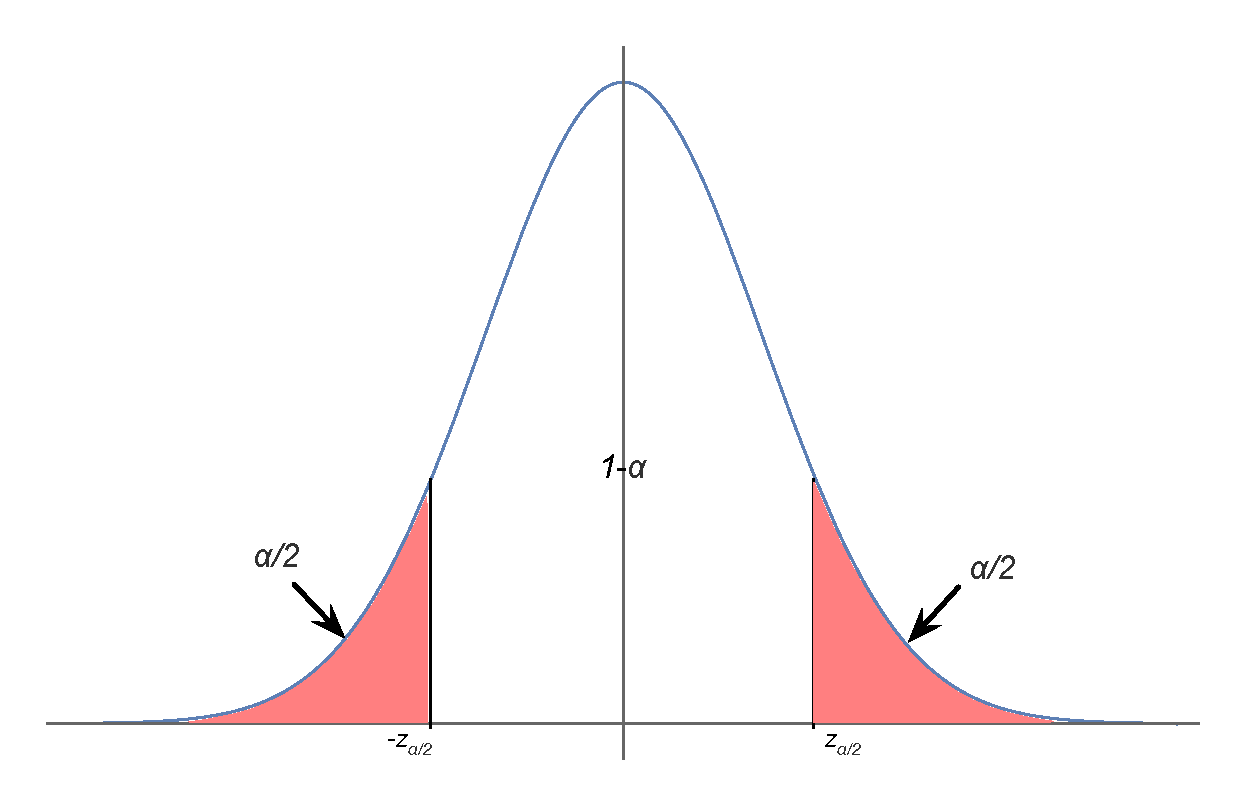
\includegraphics[width=8cm]{confidenceinterval.eps}
\end{figure}

Converting to the standard normal random variable, this is equivalent to finding values $-z_{\alpha/2}$ and $z_{\alpha/2}$ such that $\P(-z_{\alpha/2} \leq Z \leq z_{\alpha/2}) = (1 - \alpha)$. This is illustrated in the picture above. To find $-z_{\alpha/2}$ and $z_{\alpha/2}$, we can use the Z table. For example, if $(1 - \alpha) = 0.95$, then $\alpha/2 = 0.025$. Consulting the Z table, we find that $-z_{\alpha/2} = -1.96$. By symmetry of the standard normal distribution about its mean of 0, $z_{\alpha/2} = 1.96$.\\

To find our confidence interval, we convert from the standard normal distribution back to the distribution of our estimator, which is Normal$(\theta, \sigma_{\hat{\theta}})$. Substituting for $Z$, we have
\[
\P\left( -z_{\alpha/2} \leq \frac{\hat{\theta} - \theta}{\sigma_{\hat{\theta}}} \leq z_{\alpha/2} \right) = 1 - \alpha
\]
Now we just manipulate this to get it into the form we want.
\begin{align*}
\P\left( -z_{\alpha/2} \sigma_{\hat{\theta}} \leq \hat{\theta} - \theta \leq z_{\alpha/2} \sigma_{\hat{\theta}} \right) &= 1 - \alpha\\
\P\left( - \hat{\theta} -z_{\alpha/2} \sigma_{\hat{\theta}} \leq - \theta \leq -\hat{\theta} + z_{\alpha/2} \sigma_{\hat{\theta}} \right) &= 1 - \alpha\\
\P\left( \hat{\theta} - z_{\alpha/2} \sigma_{\hat{\theta}} \leq \theta \leq \hat{\theta} + z_{\alpha/2} \sigma_{\hat{\theta}} \right) &= 1 - \alpha
\end{align*}
where to get the last line we multiplied by -1 and flipped all the inequalities. Thus the $(1-\alpha)$ confidence interval for $\theta$ is:
\[
[\hat{\theta}_L, \hat{\theta}_U] = [ \hat{\theta} - z_{\alpha/2} \sigma_{\hat{\theta}}, \hat{\theta} + z_{\alpha/2} \sigma_{\hat{\theta}}]
\]
We can also write this in terms the population standard deviation $\sigma$ and the sample size $n$ by substituting $\sigma_{\hat{\theta}} = \sigma/\sqrt{n}$.
\[
[\hat{\theta}_L, \hat{\theta}_U] = \left[ \hat{\theta} - z_{\alpha/2} \frac{\sigma}{\sqrt{n}}, \hat{\theta} + z_{\alpha/2} \frac{\sigma}{\sqrt{n}}\right]
\]
Let's do some examples.

\begin{example}A ball bearing machine produces ball bearings whose diameters are normally distributed with mean $\mu$ mm and standard deviation $\sigma = 0.1$ mm. We would like to estimate the mean $\mu$ using a 90\% confidence interval. To do this, we take a sample size of $n = 9$ ball bearings and use the sample mean $\bar{Y}$ as our estimator for $\mu$. Suppose we measure $\bar{Y} = 10.0$ mm. What is the 90\% confidence interval for $\mu$?\\

Although this is not a large sample size, we can still find a confidence interval in this case because we are assuming that the population is normally distributed. Thus the sample mean $\bar{Y}$ will always be normally distributed. Since we know the population standard deviation, we can convert to the standard normal $Z$ distribution directly without appealing to approximations which require a large sample size. First compute the standard deviation of our estimator:
\[
\sigma_{\bar{Y}} = \frac{\sigma}{\sqrt{n}} = \frac{0.1}{\sqrt{9}} = \frac{0.1}{3} = 0.0333
\]
Since $1 - \alpha = 0.9$, $\alpha = 0.1$, thus $\alpha / 2 = 0.05$. Looking at the $Z$ table, we have to choose between a probability of 0.0495 ($z_{\alpha/2} = 1.65$) and a probability of 0.0505 ($z_{\alpha/2} = 1.64$). We will choose $z_{\alpha/2} = 1.65$ to allow for more ``wiggle room''. Thus our 90\% confidence interval for $\mu$ is given by:
\begin{align*}
[\bar{Y}_L, \bar{Y}_U] &= [ \bar{Y} - z_{\alpha/2} \sigma_{\bar{Y}}, \bar{Y} + z_{\alpha/2} \sigma_{\bar{Y}} ] \\
&= [ \bar{Y} - (1.65)(0.0333), \bar{Y} + (1.65)(0.0333) ] \\
&= [ 10.0 - (1.65)(0.0333), 10.0 + (1.65)(0.0333) ] \\
&= [9.945, 10.055]
\end{align*}
Although we cannot say for certain that the true population parameter $\mu$ falls within this range, we can say that the probability that it does is 0.90. If we repeated this procedure, i.e. took 9 more samples, generated the sample mean, and constructed a 90\% confidence interval, we would get a different confidence interval, but the probability that $\mu$ would fall in that confidence interval would still be 0.90.
\end{example}

Note that constructing this confidence interval required knowledge of the population standard deviation (which we then divided by $n$ to get the standard deviation of the estimator). Often we do not know this parameter, but we wish to construct a confidence interval anyway. What to we do in that case? We use the sample standard deviation (found, for example, using the estimator $S$) in place of the population standard deviation. If this sounds to you like cheating, you are right! The key is that $n$ is large. If the population is large, the sample standard deviation is close to the population standard deviation and there is very little loss of accuracy if we use $S$ in place of $\sigma$ in the formula for the confidence interval. We will justify this approximation mathematically later on, but for now just recall that the $t$ distribution (which we use when the population standard deviation is unknown) approaches the standard normal $Z$ distribution as the number of degrees of freedom increases.

\begin{example}The shopping times of $n = 64$ randomly selected customers at a local supermarket were recorded. The sample mean and sample variance of the 64 shoppers were 33 minutes and 256 minutes, respectively. Find a 98\% confidence interval for $\mu$, the true average shopping time per customer.\\

In this case, the parameter of interest is $\mu$. Our estimator is $\bar{Y}$, the sample mean. In this experiment, we sampled $n = 64$ customers and found a sample mean $\bar{Y} = 33$ and a sample variance $S^2 = 256$. Since the sample is large (more than 30 customers), by the central limit theorem, we can assume that $\bar{Y}$ is normally distributed. We do not know the population variance, so we will use the sample variance in place of the population variance. Since the population is large, this is a reasonable assumption. Thus we can use the formula above for the confidence interval, where for the standard deviation of the estimator we use:
\[
\sigma_{\bar{Y}} = \frac{S}{\sqrt{n}} = \frac{\sqrt{256}}{\sqrt{64}} = \frac{16}{8} = 2
\]
To find $z_{\alpha/2}$, we look at our Z table. Since $(1 - \alpha) = 0.98$, $\alpha = 0.02$, thus $\alpha/2 = 0.01$. Looking at our Z table, the closest probability we have to 0.01 is 0.0099 (0.0102 is the next closest, but since it is farther away, we will use 0.099), and the value of Z corresponding to that gives us $z_{\alpha/2} = 2.33$. We now have everything we need to construct our 98\% confidence interval.
\begin{align*}
[\bar{Y}_L, \bar{Y}_U] &= [ \bar{Y} - z_{\alpha/2} \sigma_{\bar{Y}}, \bar{Y} + z_{\alpha/2} \sigma_{\bar{Y}} ] \\
&= [ 33 - (2.33)(2), \bar{Y} + (2.33)(2) ] \\
&= [28.34, 37.66]
\end{align*}
\end{example}

Here is another example, this time dealing with the difference between sample proportions.

\begin{example}Two brands of lightbulbs, denoted brand A and brand B, are guaranteed to last for at least 1 year. In a random sample of 50 lightbulbs of brand A, 12 were found to fail before the 1 year period ended. In an independent random sample of 60 lightbulbs of brand B, 12 were also found to fail before the 1 year period ended. Give a 98\% confidence interval for the difference $p_1 - p_2$ between the proportion of failures of the two brands during the 1 year period.\\

The parameter of interest here is $p_1 - p_2$, and we use as our estimator $\hat{p}_1 - \hat{p}_2$. Evaluating our estimators, we get $\hat{p}_1 = 12/50 = 0.24$ and $\hat{p}_2 = 12/16 = 0.20$, thus $\hat{p}_1 - \hat{p}_2 = 0.24 - 0.20 = 0.04$. To construct our confidence interval, we need the standard deviation of our estimator. From the table above (or by deriving it from the variance of the binomial distribution), we have
\[
\sigma_{\hat{p}_1 - \hat{p}_2} = \sqrt{\frac{p_1(1-p_1)}{n_1} +\frac{p_2(1-p_2)}{n_2} }
\]
But we have a problem. The standard deviation involves the true parameter $p$, and that is what we are trying to estimate! No worries, we will just do what we did before. Since the population is large, we will use the estimator $\hat{p}$ in place of $p$ in the expression for the standard deviation.
\begin{align*}
\sigma_{\hat{p}_1 - \hat{p}_2} &\approx \sqrt{\frac{\hat{p}_1(1-\hat{p}_1)}{n_1} +\frac{\hat{p}_2(1-\hat{p}_2)}{n_2} } \\
&= \sqrt{\frac{(0.24)(0.76)}{50} +\frac{(0.20)(0.80)}{60} }\\
&= 0.0795 
\end{align*}
We found $z_{\alpha/2}$ for a 98\% confidence interval in the previous example, thus we have $z_{\alpha/2} = 2.33$. Using the formula, our 98\% confidence interval is:
\begin{align*}
[ (\hat{p}_1 - \hat{p}_2) - z_{\alpha/2} \sigma_{\hat{p}_1 - \hat{p}_2}, (\hat{p}_1 - \hat{p}_2) + z_{\alpha/2} \sigma_{\hat{p}_1 - \hat{p}_2} ] &= [ 0.04 - (2.33)(0.0795), 0.04 + (2.33)(0.0795)] \\
&= [ 0.04 - 0.185, 0.04 + 0.185] \\
&= [-0.145, 0.225]
\end{align*}
Note that our 98\% confidence overlaps 0. If the true parameter $p_1 - p_2$ were 0, then there would be no difference in the 1-year failure rates of the two brands of lightbulbs! Thus we cannot exclude that possibility with 98\% confidence.
\end{example}

\subsubsection{Experimental Design: Selecting the Sample Size}
If you are designing an experiment, one of the parameters you must choose is the sample size. As an example, suppose you are polling registered voters in Rhode Island and asking them if they are voting for Gina Raimondo. You use the estimator $\hat{p}$ for $p$, the true proportion of Raimondo voters. As the number $n$ of people polled (the size of your sample) increases, the variance of your estimator $\hat{p}$ decreases, and there is a higher probability that your estimator will be close to the true proportion. In terms of confidence intervals, if you desire 95\% confidence that your interval contains the true parameter $p$, as you increase the sample size, the confidence interval becomes narrower. There is a tradeoff, however, as the sample size gets larger. Collecting a larger sample is more expensive and consumes more resources. Is there any way mathematically to determine ahead of time the sample size we need to attain a desired level of accuracy for our estimator?\\

Suppose we want to estimate the average diameter $\mu$ of a ball bearing produced by a ball bearing machine, and we wish the probability that our estimate is within 0.02 mm of the true mean to be 0.95. Assuming the diameters of the ball bearings are normally distributed (or taking a large enough sample that the central limit theorem applies), by the 68-95-99.7 rule we want the true value $\mu$ to be within 2 standard deviations of our estimator $\bar{Y}$ (This is the standard deviation of the \emph{estimator}, not the population standard deviation). Thus we want:
\begin{align*}
2 \sigma_{\bar{Y}} = 2 \frac{\sigma}{\sqrt{n}} = 0.02 \\
\end{align*}
We can solve the above equation for $n$ as long as we know $\sigma$.
\[
n = \left( \frac{2 \sigma}{0.02}\right)^2
\]

What do we do if the population standard deviation $\sigma$ is not know, as is often the case. One possibility is to use the sample standard deviation $S$ from a previously taken sample in place of the population standard deviation $\sigma$. As long as we take a large enough sample, this is a reasonable estimate. Another alternative is to use the range (largest value minus smallest value) of a previous sample. If we assume that the population is roughly normally distributed, then we know from the 68-95-99.7 rule that 95\% of the population will lie within two standard deviations of the mean. If our sample is large enough, then the sample range should be approximately $4\sigma$, since we are assuming the range represents two standard deviations both above and below the mean. Thus we can approximate $\sigma$ as one-fourth of the range.\\

In our ball bearing example, suppose in a previous sample of 50 ball bearings we had a range of 0.4 mm. Dividing this by 4, we can estimate $\sigma = 0.4/4 = 0.1$. Plugging this info our formula above, we get:
\[
n = \left( \frac{2 \cdot 0.1}{0.02}\right)^2 = 10^2 = 100
\]

\subsection{Small Sample Confidence Intervals for Population Mean}
In this section we will discuss confidence intervals for the estimators of population means $\mu$ and $\mu_1 - \mu_2$. The confidence interval estimators in the previous section relied on the fact that the sample size was large. We used the large sample size assumption in two places. First, if the underlying sample size is not normal, we need a large sample size to apply the central limit theorem and conclude that the sample mean estimator $\bar{Y}$ is approximately normal. Second, the confidence interval formula relies on the standard deviation of the estimator, and the formula for that standard deviation involves the population standard deviation. This population standard deviation is usually unknown, so we estimate it with the sample standard deviation $S$. This approximation is only valid for a large sample size. What do we do when the sample size is small?\\

We will assume in this section that the population is normally distributed, since the sample size will be too small for the central limit theorem to apply. Let $Y_1, \dots, Y_n$ be $n$ samples from a normal population, and let $\bar{Y}$ and $S^2$ be the sample mean and variance. We would like to construct a confidence interval for the population mean $\mu$ in the case where the population variance $\sigma^2$ is unknown and the sample is too small to approximate $\sigma^2$ with $S^2$. Recall from the chapter on sampling distributions that 
\[
T = \frac{\bar{Y} - \mu}{S/\sqrt{n}}
\]
has a t-distribution with $(n-1)$ degrees of freedom. We will construct a confidence interval in the same method as for large sample sizes, but we will use the t-distribution in place of the standard normal distribution. 

\begin{figure}[H]
\centering
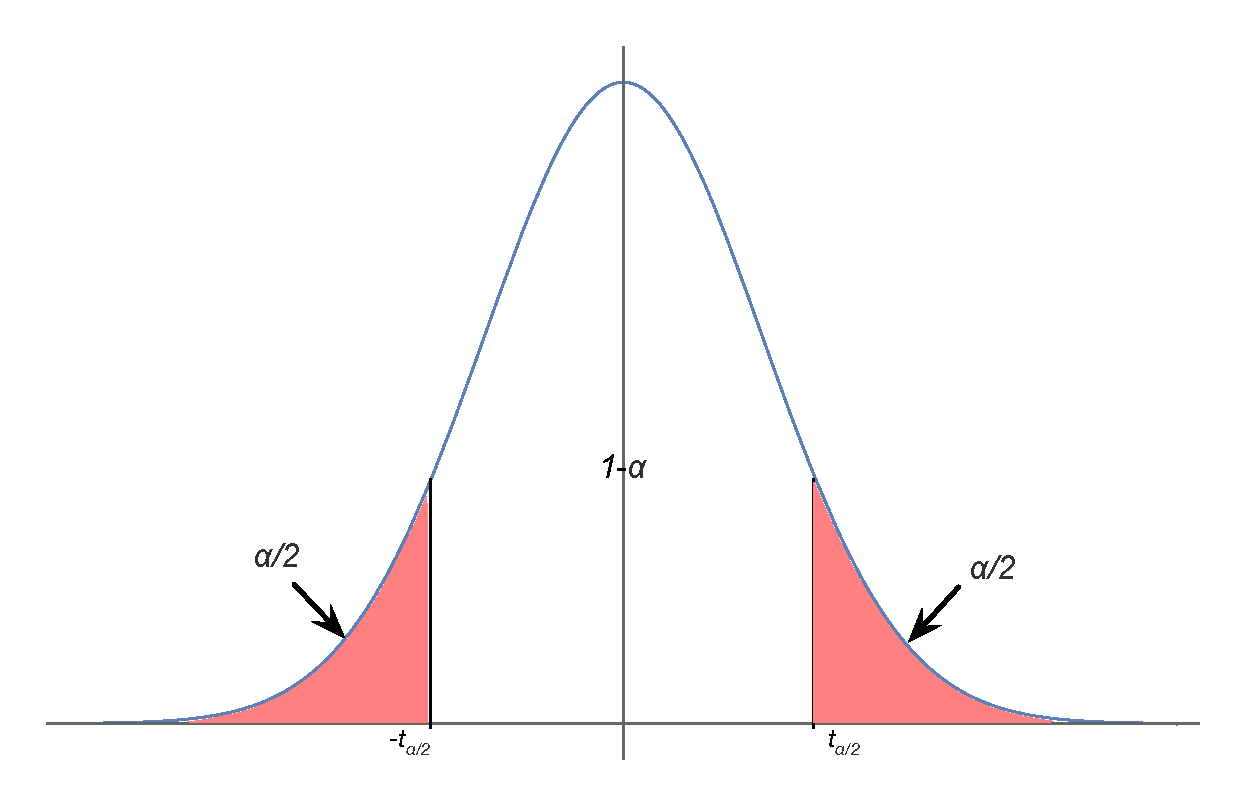
\includegraphics[width=8cm]{tconfidenceinterval.eps}
\end{figure}
As with the confidence interval involving the $Z$ distribution, given a confidence coefficient $(1 - \alpha)$, we will look for a two-sided confidence interval by dividing $\alpha$ by 2 and looking for values $-t_{\alpha/2}$ and $t_{\alpha/2}$ such that
\[
\P(-t_{\alpha/2} \leq T \leq t_{\alpha/2}) = 1 - \alpha
\]
The value $t_{\alpha/2}$ can be found from the t-table with $(n-1)$ df. The confidence interval formula is derived in exactly the same was as the large sample case, and the only differences between the formulas is that the population standard deviation $\sigma$ is replaced by the sample standard deviation $S$ and the $Z$ value is replaced by a $t$ value.
\[
[\bar{Y}_L, \bar{Y}_U] = \left[ \bar{Y} - t_{\alpha/2} \frac{S}{\sqrt{n}}, \bar{Y} + t_{\alpha/2} \frac{S}{\sqrt{n}}\right]
\]
Since the t distribution has thicker tails than the normal distribution, confidence intervals involving small sample sizes which use the t distribution will be wider than those using the $Z$ distribution.

\begin{example}You are a rocket scientist, and you conduct an experiment which involves measuring the launch velocity of a model rocket. Suppose 8 measurements are taken. The sample mean is 29.59 m/s, and the sample standard deviation is 0.391 m/s. Find a 95\% confidence interval for the true launch velocity of the model rocket.\\

We will assume that the launch velocities are normally distributed. Since we have a small sample size, we have to use the t distribution to construct our confidence interval. Since there are 8 observations, we want the t distribution with 7 df. Since $(1 - \alpha) = 0.95$, $\alpha/2 = 0.025$. From the t-table, we find that $t_{\alpha/2} = t_{0.025} = 2.365$. Thus our 95\% confidence interval is
\begin{align*}
[\bar{Y}_L, \bar{Y}_U] &= \left[ 29.59 - (2.365) \frac{0.391}{\sqrt{8}}, 25.959 + (2.365) \frac{0.391}{\sqrt{8}}\right]\\
&= \left[ 29.59 - 0.327, 29.59 + 0.327 \right]
\end{align*}
\end{example}

We can similarly handle the case where we want to compare the means of two normal populations. If the sample sizes are large and we know the standard deviations of both populations, we can use the confidence interval methods described in the previous section. If the standard deviations are not know, we will again rely on the t distribution. In this case, the algebra is a lot more messy. \emph{I think the result is interesting and useful, so I am presenting it here. It is complicated enough that I will not put it on an exam}.\\

Suppose we want to compare the means $\mu_1$ and $\mu_2$ of two populations. We will assume that they have the \emph{same} variance $\sigma_2$, but that this variance is unknown. (This assumption is important for this model.) Take a sample of size $n_1$ from the first population and a sample of size $n_2$ from the second population. Compute the sample means $\bar{Y}_1$ and $\bar{Y}_2$, and construct the estimator $\bar{Y}_1 - \bar{Y}_2$. We would like to construct a confidence interval for this estimator.
First, we compute the sample variance $S^2_1$ for the first sample and the sample variance $S^2_2$ for the second sample. An unbiased estimator for the population variance $\sigma^2$ can be obtained by pooling the sample data from both samples to obtain the \emph{pooled variance estimator} $S^2_p$:
\[
S^2_p = \frac{(n_1 - 1)S^2_1 + (n_2 - 1)S^2_2}{n_1 + n_2 - 2}
\]
This estimator is a weighted average of $S^2_1$ and $S^2_2$, with the larger sample being given a higher weight. The weights $(n_1 - 1)$ and $(n_2 - 1)$ are used in place of $n_1$ and $n_2$ so that this is an unbiased estimator (similar to the factor of $n-1$ in the denominator for the sample variance estimator $S^2$). We can show that the quantity
\[
T = \dfrac{ (\bar{Y}_1 - \bar{Y}_2) - (\mu_1 - \mu_2) }{S_p \sqrt{ \frac{1}{n_1} + \frac{1}{n_2} }}
\]
has a t distribution with $n_1 + n_2 - 2$ degrees of freedom (df). Thus, in a similar fashion to the confidence intervals we constructed earlier, the confidence interval for $(\mu_1 - \mu_2)$ is given by:
\[
\left[ (\bar{Y}_1 - \bar{Y}_2) - t_{\alpha/2} S_p \sqrt{ \frac{1}{n_1} + \frac{1}{n_2} }, (\bar{Y}_1 - \bar{Y}_2) + t_{\alpha/2} S_p \sqrt{ \frac{1}{n_1} + \frac{1}{n_2} }\right]
\]

\subsection{Consistency}
We talked in previous sections about desirable properties for estimators. Ideally, we would like our estimators to be unbiased. However, we showed in a homework problem that in certain circumstances, a biased estimator may in fact have lower mean square error (MSE) than an unbiased estimator, so bias is not the entire story. Mean square error, which is the sum of bias squared and variance, is a good measure of the accuracy of an estimator, but it does not take into account the size of the sample we are taking. Ideally, we would like to define an estimator as ``good'' if the probability of ``missing'' the true parameter value goes to 0 as the sample size gets large. This concept of ``goodness'' of an estimator is called \emph{consistency}.\\

We use the same setup as always. Consider a population which can be characterized by a parameter $\theta$. Take $n$ samples $Y_1, \dots, Y_n$ from the population, and construct from these an estimator $\hat{\theta}_n$ for $\theta$. Note the subscript $n$ indicates that we have a different estimator for each value of $n$. For example, if we want to estimate the population mean $\mu$, then we can use the sample mean as an estimator. Writing the sample mean with a subscript $n$ to denote the number of samples we are taking from our population, we have our estimator for $\mu$:
\[
\bar{Y}_n = \frac{1}{n} \sum_{i=1}^n Y_i
\]
An estimator $\hat{\theta}_n$ is \emph{consistent} for $\theta$ if the probability that $\hat{\theta}_n$ misses the true parameter by even a small amount approaches 0 as $n$ approaches infinity. Mathematically we write this as follows.

\begin{framed}
\emph{Consistency Estimator}\\
  \rule{\dimexpr\linewidth-2\fboxsep-2\fboxrule}{.1pt} \\
Let $\hat{\theta}_n$ be an estimator for a parameter $\theta$, where $\hat{\theta}_n$ is obtained from a sample of size $n$ from the underlying population. The estimator $\hat{\theta}_n$ is \emph{consistent} for $\theta$ if for all $\epsilon > 0$ (no matter how small),
\[
\lim_{n\rightarrow\infty} \P(|\hat{\theta}_n - \theta| \geq \epsilon ) = 0
\]
This type of convergence is called \emph{convergence in probability}.
\end{framed}

Like many criteria in mathematics, this is difficult to check. In the case of an unbiased estimator, we have an equivalent characterization of consistency which is much easier to verify. This is one of the reasons we like unbiased estimators, even though we have seen that unbiased estimators are not always ``better''.

\begin{framed}
\emph{Consistency of an Unbiased Estimator}\\
  \rule{\dimexpr\linewidth-2\fboxsep-2\fboxrule}{.1pt} \\
Let $\hat{\theta}_n$ be an \emph{unbiased} estimator for a parameter $\theta$, where $\hat{\theta}_n$ is obtained from a sample of size $n$ from the underlying population. Then $\hat{\theta}_n$ is consistent for $\theta$ if
\[
\lim_{n\rightarrow\infty} Var(\hat{\theta}_n) = 0
\]
\end{framed}

To see that this is true, we can use Chebyshev's Inequality. For $\epsilon > 0$, Chebyshev's Inequality gives us
\[
\P(|\hat{\theta}_n - \E(\theta)| \geq \epsilon) \leq \frac{Var(\hat{\theta}_n)}{\epsilon^2}
\]
Since $\hat{\theta}_n$ is unbiased (this is critical here), we know $\E(\theta) = \theta$, so we can substitute $\theta$ for $\E[\theta)$ above to get:
\[
\P(|\hat{\theta}_n - \theta| \geq \epsilon) \leq \frac{Var(\hat{\theta}_n)}{\epsilon^2}
\]
Taking the limit of both sides,
\[
\lim_{n\rightarrow\infty} \P(|\hat{\theta}_n - \theta| \geq \epsilon) \leq  \frac{1}{\epsilon^2} \lim_{n\rightarrow\infty} Var(\hat{\theta}_n) = 0
\]
since we are assuming that the variance of our estimator goes to 0 as $n$ goes to infinity.\\

We can apply this to see that the sample mean $\bar{Y}$ is a consistent estimator for the population mean $\mu$. Recall that the sample mean is given by:
\[
\bar{Y}_n = \frac{1}{n} \sum_{i=1}^n Y_i
\]
We have shown that this is unbiased, i.e. $\E{\bar{Y}_n} = \mu$. We also know from the section on sampling distributions that $Var(\bar{Y}_n) = \sigma^2 / n$, which goes to 0 as $n$ goes to infinity. Thus $\bar{Y}_n$ is a consistent estimator for $
\mu$. This result is known as the \emph{Weak Law of Large Numbers}, and is one of the fundamental results of probability. Recall from the beginning of the course that when we defined expected value, we said that we could think of it intuitively as taking the average of a large number of experiments. In other words, the expected value is approximately what we get if we repeat an experiment $n$ times, add up the results, and divide by $n$. The law of large numbers makes this intuition mathematically precise. $\bar{Y}_n$ is the empirical mean, i.e. what we get when we ``add-them-up-and-divide-by-$n$''. As $n$ gets large, $\bar{Y}_n$ approaches the true expected value $\mu$ in the sense that the probability that $\bar{Y}_n$ ``misses'' $\mu$ becomes arbitrarily small.\\

We can similarly show that our unbiased estimator for variance $S^2$ (which we can write $S^2_n$ to indicate the sample size of $n$) is a consistent estimator for the population variance.


\subsection{Construction of Estimators}
So far we have defined what an estimator is and discussed qualities we would like to have in our estimators (unbiased, low MSE, consistent). But we have only discussed three estimators: $\bar{Y}$, $S^2$, and $\hat{p}$. There are many more parameters we might like to estimate. How can we construct estimators for them? In this section we look at two methods of constructing estimators: the method of moments and the maximum likelihood estimator (MLE).

\subsubsection{Method of Moments}
This method is based on the fact that the sample mean $\bar{Y}$ is a consistent estimator for the population mean $\mu$. A population parameter is often a function of the population mean. For example, if we have a population which has a Poisson distribution, then the Poisson parameter $\lambda$ is equal to the population mean $\mu$. Thus we can estimate $\lambda$ by the sample mean $\bar{Y}$, i.e. $\hat{\lambda} = \bar{Y}$ is an estimator for the Poisson parameter $\lambda$.\\

In its most simple form, the method of moments works as follows:
\begin{enumerate}
\item Write the parameter of interest in terms of the population mean, i.e. solve for the parameter in terms of the population mean $\mu$.
\item Substitute $\bar{Y}$ for $\mu$ to get the method of moments estimator.
\end{enumerate} 

Let's do some examples.

\begin{example}Suppose we have a population which has a uniform distribution on the interval $[0, b]$. Find the method of moments estimator for $b$.\\

The population mean $\mu$ is the expected value of a uniform random variable, so $\mu = \frac{b-0}{2} = \frac{b}{2}$. Solving for $b$ we get $b = 2 \mu$. Substituting $\bar{Y}$ for $\mu$ we get $b = 2 \bar{Y}$. Thus our method of moments estimator for $b$ is:
\[
\hat{b} = 2 \bar{Y}
\]

Since $\E(\bar{Y}) = \mu$, $\hat{b}$ is an unbiased estimator for $b$. What is its variance?
\begin{align*}
Var(\hat{b}) &= Var(2 \bar{Y} ) \\
&= 4 Var(\bar{Y}) \\
&= 4 \frac{\sigma^2}{n} \\
&= 4 \frac{b^2}{12n} \\
&= \frac{b^2}{3n}
\end{align*}
where we used both the variance of $\bar{Y}$ and the variance of the uniform distribution on $[0, b]$. Since there is a factor of $n$ in the denominator, the variance of $\hat{b}$ goes to 0 as $n$ goes to infinity, thus the method of moments estimator is a consistent estimator for $b$.\\
\end{example}

\begin{example}Suppose we have a population which has a geometric distribution with parameter $p$. Find the method of moments estimator for $p$.\\

The population mean $\mu$ is the expected value of a geometric random variable, so $\mu = 1 / p$. Solving for $p$, we get $p = 1 / \mu$. For the method of moments, we substitute $\bar{Y}$ for $\mu$, thus the method of moments estimator is:
\[
\hat{p} = \frac{1}{\bar{Y}}
\]
\end{example}

\begin{example}Suppose we have a population which has a Poisson distribution with parameter $\lambda$. Find the method of moments estimator for $\lambda$.\\

Since the population mean is $\mu = \lambda$, the method of moments estimator is $\hat{\lambda} = \bar{Y}$.
\end{example}

Sometimes we cannot construct an method of moments estimator in this way, i.e. we cannot solve for the parameter in terms of the population mean $\mu$. For example, suppose the population is uniformly distributed on $[a, b]$, and we want to estimate both $a$ and $b$. The population mean is $\mu = \frac{a + b}{2}$, but we cannot solve for either $a$ or $b$ in terms of $\mu$ without having an expression in terms of the other parameter. The idea here is to estimate the variance using the method of moments, and then we have two equations for the two unknowns $a$ and $b$. Since the algebra gets messy really quickly, we will not be pursuing this any further. All method of moments estimators we will use will only involve the sample mean $\bar{Y}$.

\subsubsection{Maximum Likelihood Estimator (MLE)}
The method of moments is very intuitive but often does not lead to the best estimators. A second way of constructing estimators is called the maximum likelihood estimator (MLE). Let's look an an example to illustrate how the MLE works.

\begin{example}You have a bag which contains three marbles. You know they are either red or white, but you do not know how many of each are in the bag. For some reason, you are forbidden from opening the bag and looking at the marbles. However, you are permitted to sample two marbles without replacement. Suppose we draw out two red balls. What is a good estimate of the number of red balls in the bag?\\

Since we drew two red balls, the bag either contains two red balls or three red balls. If the bag contains two red balls, then the probability of our draw is:
\[
\dfrac{\binom{2}{2}\binom{1}{0}}{\binom{3}{2}} = \frac{1}{3}
\]
If the bag contains three red balls, then the probability of our draw is:
\[
\dfrac{\binom{3}{2}}{\binom{3}{2}} = 1
\]
A reasonable estimate for the number of red balls in the bag is 3, since that maximizes the probability of our draw.
\end{example}
The method illustrated in the example above is known as the method of \emph{maximum likelihood}, since we choose the parameter which maximizes the probability of attaining our sample. Before we give the formal definition and more examples, we need to formally define the concept of likelihood.\\

Suppose we have a population whose distribution can be characterized by a parameter $\theta$. The pmf or density function for the population will depend on $\theta$, so the parameter $\theta$ will appear in the formula for the pmf or density function. We will indicate this dependence on $\theta$ as a subscript $\theta$. Let $p_\theta(y)$ or $f_\theta(y)$ be the pmf or density function for our population. Now take a sample of size $n$, denoted $Y_1, Y_2, \dots, Y_n$, from our population. Then we define the \emph{likelihood} of our sample as follows.

\begin{framed}
\emph{Likelihood of a Sample}\\
  \rule{\dimexpr\linewidth-2\fboxsep-2\fboxrule}{.1pt} \\
Let $Y_1, Y_2, \dots, Y_n$ be a sample drawn from a population with pmf or density $p_\theta(y)$ or $f_\theta(y)$. Then the \emph{likelihood} of the sample is given by:
\begin{align*}
L(Y_1, Y_2, \dots, Y_n|\theta) &= p_\theta(Y_1) p_\theta(Y_2) \cdots p_\theta(Y_n) & \text{discrete distribution}\\
L(Y_1, Y_2, \dots, Y_n|\theta) &= f_\theta(Y_1) f_\theta(Y_2) \cdots f_\theta(Y_n) & \text{continuous distribution}
\end{align*}
In other words, we plug the samples into the pmf or density and multiply them together.
\end{framed}
The maximum likelihood estimator (MLE) chooses the value of the parameter $\theta$ which maximizes the likelihood of our sample.
\begin{framed}
\emph{Maximum Likelihood Estimator}\\
  \rule{\dimexpr\linewidth-2\fboxsep-2\fboxrule}{.1pt} \\
Let $Y_1, Y_2, \dots, Y_n$ be a sample drawn from a population parameterized by $\theta$, and let $L(Y_1, Y_2, \dots, Y_n|\theta)$ be the likelihood of the sample. Then the \emph{maximum likelihood estimator} (MLE) for $\theta$, which is sometimes written $\hat{\theta}_{MLE}$, is the value of $\theta$ which maximizes the likelihood $L(Y_1, Y_2, \dots, Y_n|\theta)$.
\end{framed}

Let's do some examples of this. We will redo the three examples from the method of moments section.

\begin{example}Suppose we have a population which has a uniform distribution on the interval $[0, b]$. Take a sample $Y_1, \dots, Y_n$ from this distribution. Find the MLE for $b$.\\

First we need to find the likelihood function $L(Y_1, \dots, Y_n|b)$. The density function for a uniform distribution on $[0, b]$ is
\[
f_\theta(y) = \begin{cases}
\frac{1}{b} & 0 \leq y \leq b \\
0 & \text{otherwise}
\end{cases}
\]
Thus the likelihood function is 
\begin{align*}
L(Y_1, Y_2, \dots, Y_n|\theta) &= f_\theta(Y_1) f_\theta(Y_2) \cdots f_\theta(Y_n) \\
&= \begin{cases}
\frac{1}{b^n} & \text{if $0 \leq Y_i \leq b$ for all samples $Y_i$} \\
0 & \text{otherwise, i.e. if for any sample $Y_i > b$ or $Y_i < 0$ }
\end{cases}
\end{align*}
The MLE is the value of $b$ which maximizes this likelihood function. We do not want the likelihood to be 0, since that cannot be a maximum, thus we need to have $0 \leq Y_i \leq b$ for all samples $Y_i$. Since $b$ is in the denominator in our expression above, to maximize the likelihood we want to make $b$ as small as possible without causing the likelihood to be 0. In other words, we want the \emph{narrowest} interval for the uniform distribution that we can get away with, i.e. the smallest value for $b$ for which the interval can contain our sample points. How do we do this? If we choose $b$ to be the largest of our sample points, we have maximized our likelihood! In other words, our MLE estimator is the largest order statistic of our data:
\[
\hat{b}_{MLE} = \max(Y_1, Y_2, \dots, Y_n) = Y_{(n)}
\]
This is very different from our method of moments estimator above. Is this estimator unbiased? The expected value of this estimator is a little tricky to compute, but we can do it if we think in terms of CDFs. Let $Y \sim$ Uniform$[0, b]$, and let $F(y)$ be the CDF of $Y$, i.e. $F(y) = \P(Y \leq y)$. Let $Y_{(n)} = \max(Y_1, Y_2, \dots, Y_n)$, and let $F_{(n)}$ be the CDF for $Y_{(n)}$. Then
\begin{align*}
F_{(n)}(y) &= \P(Y_{(n)} \leq y) \\
&= \P(\max(Y_1, Y_2, \dots, Y_n) \leq y) \\
&= \P(Y_i \leq y \text{ for all $i = 1, \dots, n$}) \\
&= F(Y_1)F(Y_2)\dots F(Y_n)
\end{align*}
We can get the CDF of $Y$ by integrating the uniform density:
\[
F(y) = \begin{cases}
0 & y < 0 \\
\frac{y}{b} & 0 \leq y \leq b \\
1 & y > 1
\end{cases}
\]
Thus as long as all the samples are in the interval $[0, b]$ we have
\[ 
F_{(n)}(y) = \left( \frac{y}{b} \right)^n
\]
To get the density $f_{(n)}$ of $Y_{(n)}$ we take the derivative of the CDF with respect to $y$.
\begin{align*}
f_{(n)}(y) &= \frac{d}{dy}F_{(n)}(y) \\
&= n y^{n-1} \frac{1}{b^n}
\end{align*}
The density is 0 outside the interval $[0, b]$, so with the appropriate limits the density becomes
\begin{align*}
f_{(n)}(y) = \begin{cases}
n y^{n-1} \frac{1}{b^n} & 0 \leq y \leq b \\
0 & \text{otherwise}
\end{cases}
\end{align*}
So to get the expected value of $Y_{(n)}$ we use the formula for the expected value of a continuous random variable.
\begin{align*}
\E( Y_{(n)} ) &= \int_0^b y f_{(n)}(y) dy\\
&= \int_0^y y n y^{n-1} \frac{1}{b^n} \\
&= \frac{n}{b^n} \int_0^b y^n dy \\
&= \frac{n}{b^n} \frac{y^{n+1}}{n+1}\Bigr|_0^b \\
&= \frac{n}{b^n} \frac{b^{n+1}}{n+1} \\
&= \frac{n}{n+1} b 
\end{align*}
Since this is not equal to $b$, the MLE is a biased estimator for the parameter $b$. However, we can convert this to an unbiased estimator by multiplying it by $(n+1)/n$. Thus the estimator
\[
\frac{n+1}{n}Y_{(n)} = \frac{n}{n+1} \max(Y_1, Y_2, \dots, Y_n)
\]
is an unbiased estimator for $b$.

\end{example}

\begin{example}Suppose we have a population which has a geometric distribution with parameter $p$. Take samples $Y_1, \dots, Y_n$ from this distribution. Find the MLE for $p$.

Recall that the pmf for the geometric distribution with parameter $p$ is:
\[
p(k) = \mathbb{P}(Y = k) = (1 - p)^{k-1} p
\]
Then our likelihood function is:
\begin{align*}
L(Y_1, \dots, Y_n | p) &= \prod_{i = 1}^n (1 - p)^{Y_i-1} p
\end{align*}

To maximize this, we need to use calculus. We will differentiate with respect to $p$ and set the derivative equal to zero. Since this requires an annoying amount of algebra, we will use a trick. Since the log function is strictly increasing, the log of the likelihood function and the likelihood function attain their maximum at the same value of $p$. So we can find the maximum of the log likelihood function instead, and this will give us the correct maximum for $p$.
\begin{align*}
\log L(Y_1, \dots, Y_n | p) &= \log \prod_{i = 1}^n (1 - p)^{Y_i-1} p \\
&= \sum_{i = 1}^n \log p + \sum_{i = 1}^n \log (1 - p)^{Y_i-1} \\
&= n \log p +  \sum_{i = 1}^n (Y_i-1) \log (1 - p)
\end{align*}
Taking the derivative with respect to $p$:
\[
\frac{d}{dp} \log L(Y_1, ..., Y_n | p) = \frac{n}{p} - \frac{1}{1 - p} \left( \sum_{i = 1}^n Y_i - n \right)
\]
For this to be 0 we require:
\begin{align*}
 \frac{1}{1 - p} \left( \sum_{i = 1}^n Y_i - n \right) &= \frac{n}{p} \\
p \left( \sum_{i = 1}^n Y_i - n \right) &= n(1-p) \\
p \sum_{i = 1}^n Y_i - np &= n - np \\
p &= \frac{n}{\sum_{i = 1}^n Y_i } = \frac{1}{\bar{Y}}
\end{align*}
Thus the MLE for the parameter $p$ is $1/\bar{Y}$. This is the same estimator as we found by the method of moments above.

\end{example}

\begin{example}Suppose we have a population which has a Poisson distribution with parameter $\lambda$. Take samples $Y_1, \dots, Y_n$ from this distribution. Find the MLE for $\lambda$.\\

Using the Poisson pmf, The likelihood function is:
\begin{align*}
L(Y_1, \dots, Y_n | \lambda) &= \prod_{i=1}^n \frac{e^{-\lambda} \lambda^{Y_i}}{Y_i!} \\
&= e^{-n \lambda} \lambda^{\sum_{i=1}^n Y_i} \prod_{i=1}^n \frac{1}{Y_i!} \\
&= e^{-n \lambda} \lambda^{n \bar{Y}} \prod_{i=1}^n \frac{1}{Y_i!} \\
\end{align*}
To maximize this with respect to $\lambda$, we will maximize the log likelihood function.
\begin{align*}
\log L(Y_1, \dots, Y_n | \lambda) &= \log(e^{-n \lambda}) + \log(\lambda^{n \bar{Y}} ) + \log \left( \prod_{i=1}^n \frac{1}{Y_i!}  \right)\\
&= -n \lambda + n \bar{Y} \log(\lambda) + \log \left( \prod_{i=1}^n \frac{1}{Y_i!} \right)
\end{align*}
Taking the derivative with respect to $\lambda$:
\begin{align*}
\frac{d}{d \lambda} \log L(Y_1, \dots, Y_n | \lambda) &= -n + \frac{ n \bar{Y} }{\lambda}
\end{align*}
Setting this equal to 0, we get $\lambda = \bar{Y}$, which is the same estimator we got using the method of moments.
\end{example}


\end{document} 
